

We consider the following advection problem taken from \cite[ex 5.2]{li06}:
\[
\frac{\partial T}{\partial t} + u \frac{\partial T}{\partial x} = 0
\]
for $x\in [0,1]$ and with the initial conditions:
\[
T(x,0)=
\left\{
\begin{array}{ll}
\sin (10 \pi x) & \textrm{for } x\leq 0.1 \\
0               & \textrm{for } x\geq 0.1 
\end{array}
\right.
\]
The velocity is set to $u=0.1$.
We use 200 elements and a time step of $\delta t=10^{-4}$. 
We run the model to time $t=8$ so we need 80,000 time stpes. 
Note that the CFL-number is then very small: 
\[
C = \frac{\delta t \cdot u}{h} = \frac{10^{-4} \cdot  0.1}{1/200} = 0.002
\]

\begin{center}
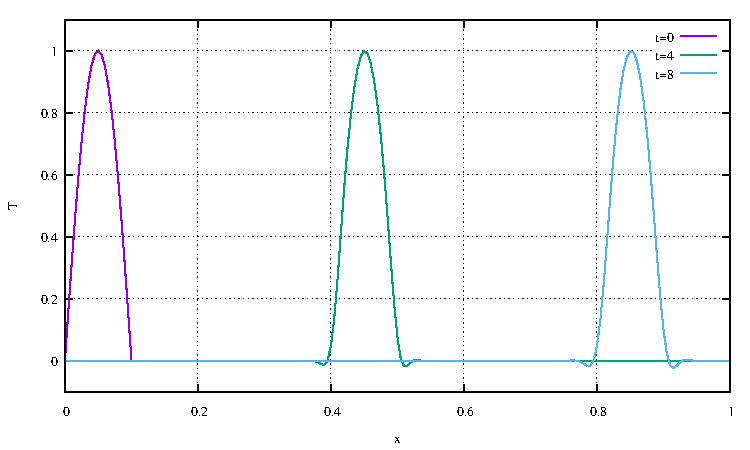
\includegraphics[width=9cm]{python_codes/fieldstone_60/results/T.pdf}\\
{\captionfont Temperature field at three different times.}
\end{center}




